\chapter{TEMEL BİLGİLER} \label{chapter:temelBilgiler}
Tez çalışması boyunca kullanılan teknolojiler hakkında temel bilgiler bu bölümde sunulmuştur.
\section{FPGA Platformu}
%FPGA'ler birbirlerine programlanabilir bağlantı birimleriyle bağlı matris yapıda özelleştirilebilir mantık bloklarından (Configurable Logic Block/CLB) oluşan programlanabilir yarı iletken devrelerdir. FPGA’ler herhangi bir uygulama için kolayca programlanabilir, aynı FPGA içeriği değiştirilip tekrar programlanarak bir başka uygulama için de kullanılabilir. Bir FPGA’in lojik hücrelerinden oluşan iç mimarisi teorik olarak Şekil \ref{image:fpgaCLB}’de verilmiştir.
%\begin{figure}[h]
%\centering
%\shorthandoff{=}
%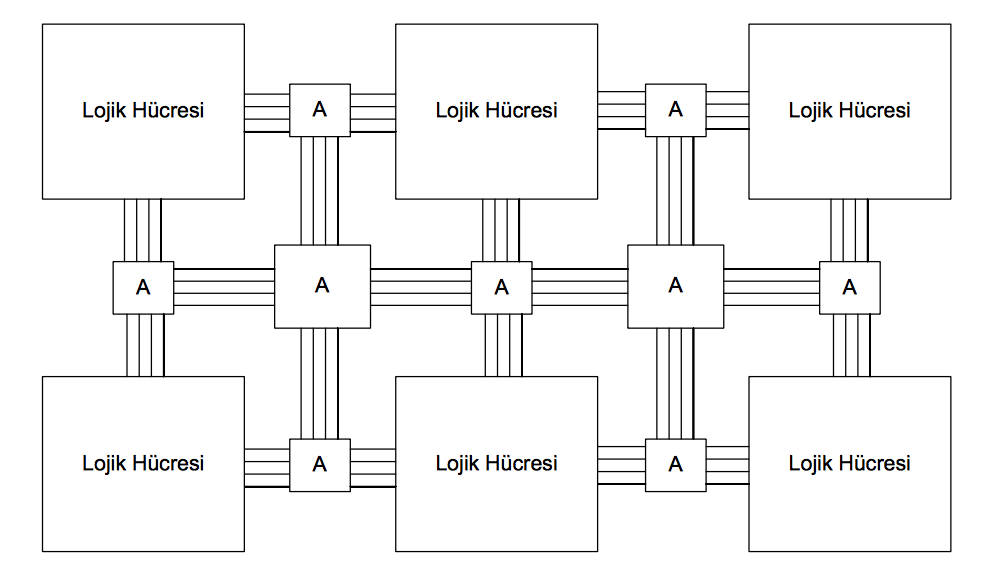
\includegraphics[width=0.8\textwidth]{gorsel/fpgaCLB.png}
%\shorthandoff{=}
%\caption{FPGA Mantık Hücreleri ve Bağlantı Yapısı}
%\label{fpgaCLB}
%\end{figure}

%FPGA'ler esnek mimari yapıları ve programlanma özellikleri sayesinde kendilerine endüstride hızla yer bulmuşlardır ve günümüzde de otomotivden, telekomünikasyona, uzay uygulamalarından savunma sanayine ve özellikle yüksek performansla birlikte esneklik isteyen birçok uygulama alanında tercih edilmektedirler.\par
Xilinx ve Altera firmaları dünya üzerinde en çok müşteriye sahip iki firmadırlar. Bu firmalar birçok uygulamaya özel ve farklı ihtiyaçlara hitap eden değişik FPGA aileleri üretmektedirler. Xilinx firmasının piyasada sıklıkla kullanılan farklı FPGA ailelerinden FPGA örnekleri ve özellikleri tablo \ref{table:fpgaModels}’de verilmiştir.
\begin{longtable}{p{100pt} p{250pt}}
\caption{Xilinx FPGA Kaynak Durumları} \label{table:fpgaModels} \\
\multicolumn{1}{c}{} & 
\multicolumn{1}{c}{\textbf{Logic Slice}} & 
\multicolumn{1}{c}{\textbf{Block RAM (kb)}} &
\multicolumn{1}{c}{\textbf{DSP Slice}} & 
\multicolumn{1}{c}{\textbf{User I/O}} &
\\ 
\hline 
\endfirsthead

\multicolumn{2}{c}%
{{\bfseries \tablename\ \thetable{} -- devam}} \\
\multicolumn{1}{c}{} & 
\multicolumn{1}{c}{\textbf{Logic Slice}} & 
\multicolumn{1}{c}{\textbf{Block RAM (kb)}} &
\multicolumn{1}{c}{\textbf{DSP Slice}} & 
\multicolumn{1}{c}{\textbf{User I/O}} &
\\  \hline 
\endhead

\hline \multicolumn{2}{r}{{Sonraki sayfada devam etmektedir.}} \\ 
\endfoot

\hline \hline
\endlastfoot
  Spartan-3A CX3S200A  &   4032 &   288 &  16  &  248 \\
  Spartan-3A CX3S1400A &  25344 &   576 &  32  &  502 \\
  Virtex-5 XC5VLX50    &   9600 &  1152 &  32  &  400 \\
  Virtex-5 XC5VLX330   & 103680 & 10368 &  192 & 1200 \\
  Virtex-7 XC7V585T    & 182100 & 28620 & 1260 &  850 \\
  Virtex-7 XC7V2000T   & 305400 & 46512 & 2160 & 1200 \\
\end{longtable}

Mantık hücresi (Logic Slice) olarak isimlendirilen birimler FPGA’lerin temel işlem ve depolama birimlerini içermektedirler. Bir mantık hücresinin içerisinde temel olarak 4 ya da daha fazla girişli lookup table (LUT), bir adet flip flop ve çeşitli çoklayıcılar (multiplexer) bulunmaktadır. Basitçe doğruluk tablosu oluşturulabilen sade devreler bir adet mantık hücresi kullanılarak gerçeklenebilir. Fakat karmaşık mantık yapısına ve çokça kaydedici yazmaca (register) ihtiyacı olan devreler ancak birden çok mantık hücresi kullanılarak gerçeklenebilirler. Sürekli gelişmekte olan FPGA teknolojisinde artık FPGA yongalarının içerisine özel fonksiyona sahip makro birimler yerleştirilmektedir. Bu makro birimler hard olarak yongaya gömülü durumda olup sadece izin verilen ölçüde parametreleri programlanabilmektedirler. Bu makro bloklara örnek olarak DCM, RAM, DSP slice, çarpıcı birimleri gösterilebilir. Genel olarak bir FPGA’in mimari yapısı şekil \ref{image:fpgaGenelMimari}’de görülebilir.
\begin{figure}[h]
\centering
\shorthandoff{=}
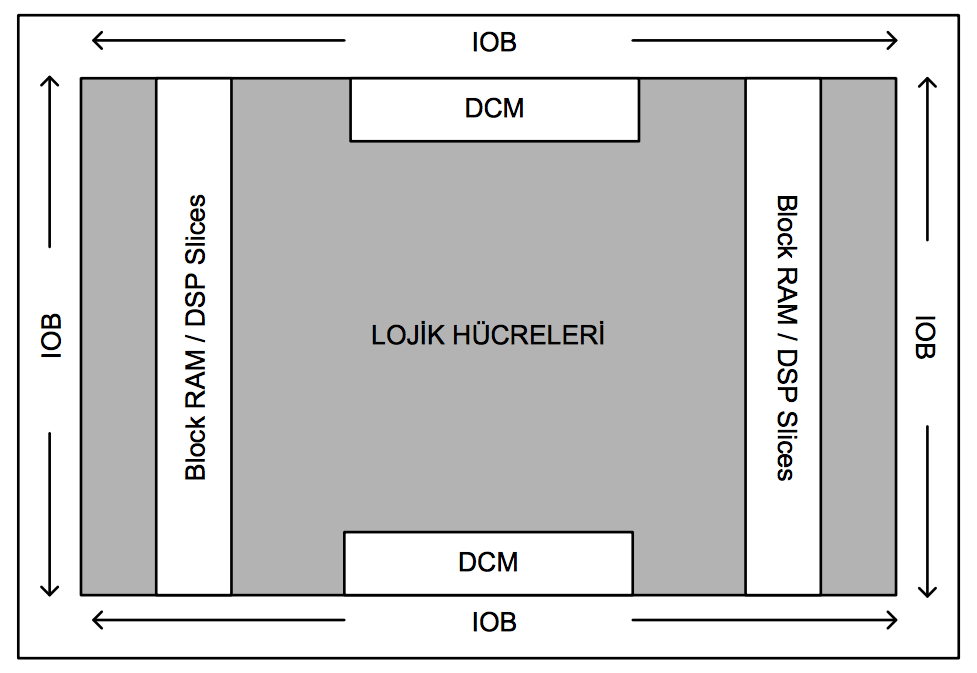
\includegraphics[width=0.8\textwidth]{gorsel/fpgaGenelMimari.png}
\shorthandoff{=}
\caption{FPGA Genel Mimari Yapısı}
\label{fpgaGenelMimari}
\end{figure}
Bu tez çalışması için Xilinx Virtex 7 ailesinden XC7VX690T FPGA’i seçilmiştir. Bu FPGA içinde 108300 slice, 693120 mantık hücresi 866400 CLB flip flop, 10888 KB dağınık ram, 1470 adet 36kbit block ram primitive vardır. \par

\section{GPGPU}

GPU teknolojisindeki ilerlemelerle birlikte, günümüzde kullanılan modern GPU’lar programlanabilir arayüzler sunar hale gelmişlerdir. Bu programlanabilir arayüzler sayesinde GPU’nun işlem gücü ve paralel işleyebilme yeteneği sadece grafik işlemlerinde değil aynı zamanda genel amaçlı hesaplamalarda da kullanılabilir hale gelmiştir. Bu durum ortaya grafik işlem birimi üzerinde genel amaçlı hesaplama (GPGPU - General Purpose programming on Graphic Processing Unit) kavramını çıkarmıştır. \par
GPU’lar yukarıdaki kısımlarda açıklanan işlem hattı mimarisi sayesinde, paralel olarak işlenebilecek nitelikte verinin yüksek performanslı bir şekilde paralel olarak işlenmesi konusunda çok elverişlidirler. GPGPU uygulamaları GPU’ların grafik aygıtlarına özel olan köşe kenar dönüşümü, dokulandırma, renklendirme, gölgelendirme vb. özelliklerinden ziyade SIMD şeklinde çalışan işlem hattı mimarisinden yararlanırlar. GPGPU uygulamaları genel olarak; işaret işleme, ses işleme, görüntü işleme, şifreleme, bioinformatik, yapay sinir ağları, paralelleştirilebilen bilimsel hesaplamalar, istatiksel hesaplamalar gibi yüklü miktarda verinin küçük parçaları üzerinde bağımsız ve paralel olarak işlem yapılmasına uygun olan uygulama alanlarında başarılıdırlar.\par

GPGPU uygulamaları genel olarak CPU üzerinde çalışan bir host program ve GPU’daki çekirdekler üzerinde hesaplama yapacak olaran çekirdek fonksiyonundan (kernel function) oluşur. Her çekirdekte çalışan çerkirdek fonksiyonu, stream şekilde GPU’ya iletilen verinin kendine düşen daha küçük bir birimi üzerinde işlem yapar. Giriş verisinin GPU’ya iletilmesi, sonuç verisinin toplanması istenilen formata dönüştürülmesi gibi ardışık işlemleri CPU’da çalışan host program yürütür. \par
şekil \ref{cudaProgrammingStructure}’da modern GPGPU dillerinden CUDA programlama diline ait programlama modeli yapısı \cite{cudaProgrammingStructure},  tablo \ref{table:cudaCComparision}’de ise C programlama diliyle yazılmış CPU üzerinde çalışan bir matris toplama fonksiyonu ile yine aynı matris toplama fonksiyonunu GPU üzerinde gerçekleyen, CUDA programlama diliyle yazılmış GPU üzerinde çalışan bir kernel fonksiyonu ve C’de yazılmış bir host program gösterilmiştir. şekil \ref{cudaProgrammingStructure}’da görüldüğü üzere, CUDA programlama modelinde GPU aygıtı grid olarak görülür ve çok sayıda bloktan oluşur. GPU’da bulunan çok sayıdaki çekirdekten her biri aynı anda bir blok işleyebilir. Bir blok içerisinde paralel olarak çalıştırılabilen çok sayıda thread bulunur. Bu ipliklerinin her biri kendisine düşen veri öbeği üzerinde tanımlanmış olan çekirdek fonksiyonu çalıştırır.

\begin{figure}[h]
\centering
\shorthandoff{=}
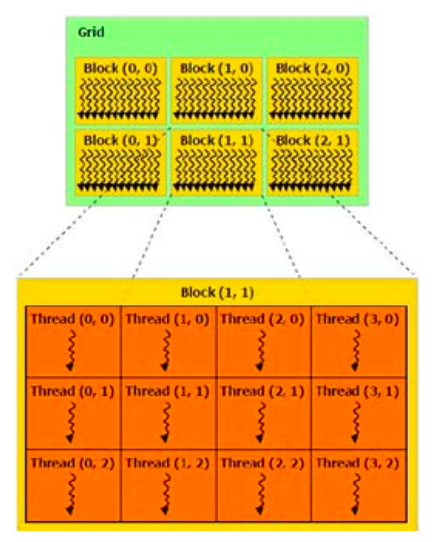
\includegraphics[width=0.8\textwidth]{gorsel/cudaProgrammingStructure.png}
\shorthandoff{=}
\caption{CUDA programlama modeli}
\label{cudaProgrammingStructure}
\end{figure}

\begin{longtable}{p{100pt} p{250pt}}
\caption{Matris Toplama İşleminin C ve CUDA'da Gerçeklenmesi} \label{table:cudaCComparision} \\
\multicolumn{1}{c}{\textbf{CPU C Programı}} & \multicolumn{1}{c}{\textbf{CUDA C Programı}} \\ 
\hline 
\endfirsthead

\multicolumn{2}{c}%
{{\bfseries \tablename\ \thetable{} -- devam}} \\
\multicolumn{1}{c}{\textbf{CPU C Programı}} & \multicolumn{1}{c}{\textbf{CUDA C Programı}} \\ 
\hline 
\endhead

\hline \multicolumn{2}{r}{{Sonraki sayfada devam etmektedir.}} \\ 
\endfoot

\hline \hline
\endlastfoot
  void add_matrix_cpu (float *a, float *b, float *c, int N){  & _global_ void add_matrix_gpu (float *a, float *b, float *c, int N){ \\
    int i,j,index;                                            & int i = blockIdx.x*blockDim.x+threadIdx.x; \\
    for (i = 0 ; i < N ; i++){                                & int y = blockIdx.y*blockDim.y+threadIdx.y; \\
      for (j = 0 ; j < N ; j++){                              & int index = j+i*N; \\
        index = j+i*N;                                        & if (i<N && j<N)  \\
        c[index] = a[index] + b[index];                       &  c[index] = a[index] + b[index]; \\
      }                                                       &} \\
    } & \\
  } & \\
  & \\
  void main(){                    &  void main () { \\
    ...                           &  dim3 dimBlock(blocksize,blocksize);  \\
    add_matrix (a,b,c,N);         &  dim3 dimGrid(N/dimBlock.x,N/dimBlock.y);  \\
    ...                           &  add_matrix_gpu << dimGrid , dimBlock >> (a,b,c,N); \\
  } & }\\
\end{longtable}

Tablo \ref{table:cudaCComparision}’de görüldüğü gibi C programlama dilinde yazılmış olan matris toplama fonksiyonu matris elemanları üzerinde ardışık döngüler şeklinde işlem yaparak matris toplama işlemini gerçekleştirir. CUDA ile yazılmış matris toplama programına bakıldığında, program CPU üzerinde çalışan host programdaki main fonksiyonundan ve GPU üzerinde çalışan add_matrix_gpu çekirdek fonksiyonundan oluşur. Host program bir bloğun boyutunu ve grid içerisindeki blok sayısını belirler. Daha sonra bloklar üzerinde paralel olarak çalışacak olan add_matrix_gpu fonksiyonunu çağırır. çağrı sonucu add_matrix_gpu çekirdek fonksiyonu bloklar ve bloklardaki threadler üzerinde paralel olarak yürütülür. Her bir thread kendi thread numarası (thread ID), blok numarası (block ID) ve blok boyutunu (blockDim) kullanarak kendine düşen veri parçası için matris toplama işlemini gerçekleştirir. \par


